%-----------------------------------------------------------------------
%\subsection{Mode and Level}
%-----------------------------------------------------------------------
%\tbc
%Baseliyos Jacob

\section{System Architecture view in ERA TSI Subset 25 Chapter 2 "Basic System Description"}
The system architecture is an outcome on the functional decomposition according to the analysis of the document in § 2 Input documents. A starting point for the first analysis is the System Strcuture in ERA TSI Subset 26 chapter 2 the subchapter 2.5 and 2.4.\\

Since we decided in the openETCS project not to consider all subsystem due to our using scope for the proof of concept on the ETCS Level 2 Utrecht - Amsterdam line, we analysed the necessary subsystem as seen here:\\

\subsection{System Structure from the subchapter 2.4. of ERA TSI Subset 26 chapter 2}

\begin{itemize}
\item 2.4.1.1	Due to the nature of the required functions, the ERTMS/ETCS system will have to be partly on the trackside and partly on board the trains. 
\item 2.4.1.2	This defines two sub-systems, the on-board sub-system and the trackside sub-system.
2.4.1.3	The environment of ERTMS/ETCS system is composed of:
\item a)	the train, which will then be considered in the train interface specification;
\item b)	the driver, which will then be considered via the driver interface specification;
\item c)	other onboard interfaces (see architecture drawing in 2.5.3),
\item d)	external trackside systems (interlockings, control centres, etc.), for which no 
\item interoperability requirement will be established.
\end{itemize}

\subsection{Sub System from the subchapter 2.5. of ERA TSI Subset 26 chapter 2}
\subsubsection{2.5.1 Trackside subsystem}
\paragraph{§ 2.5.1.1	Depending of the application level (see further sections), the trackside sub-system can be composed of:}
\begin{itemize}
\item a) balise
\item b) lineside electronic unit \textbf{\textit{- not in the scope of this project}}
\item c) the radio communication network (GSM-R)
\item d) the Radio Block Centre (RBC)
\item e) Euroloop \textbf{\textit{- not in the scope of this project}}
\item f) Radio infill unit \textbf{\textit{- not in the scope of this project}}
\item g) Key Management Centre (KMC) \textbf{\textit{- not in the scope of this project}}
\end{itemize}


\paragraph{2.5.1.2 Balise}
\begin{itemize}
\item 2.5.1.2.1	The balise is a transmission device that can send telegrams to the on-board sub-system.
\item 2.5.1.2.2	The balise is based on the existing Eurobalise specifications. These documents are included in the frame of the ERTMS/ETCS specifications.
\item 2.5.1.2.3	The balises provides the up-link, i. e. the possibility to send messages from trackside to the on-board sub-system.
\item 2.5.1.2.4	The balises can provide fixed messages or, when connected to a lineside electronic unit, messages that can be changed. 
\item 2.5.1.2.5	The balises will be organised in groups, each balise transmitting a telegram and the combination of all telegrams defining the message sent by the balise group.
\end{itemize}

\paragraph{2.5.1.3 Lineside electronic unit \textit{- not in the scope of this project}}
\begin{itemize}
\item 2.5.1.3.1	The lineside electronic units are electronic devices, that generate telegrams to be sent by balises, on basis of information received from external trackside systems.
\end{itemize}

\paragraph{2.5.1.4 Trackside radio communication network (GSM-R)}
\begin{itemize}
\item 2.5.1.4.1	The GSM-R radio communication network is used for the bi-directional exchange of messages between on-board sub-systems and RBC or radio infill units. 
\item 2.5.1.4.2	Intentionally deleted
\end{itemize}

\paragraph{2.5.1.5 RBC}
\begin{itemize}
\item 2.5.1.5.1	The RBC is a computer-based system that elaborates messages to be sent to the train on basis of information received from external trackside systems and on basis of information exchanged with the on-board sub-systems. 
\item 2.5.1.5.2	The main objective of these messages is to provide movement authorities to allow the safe movement of trains on the Railway infrastructure area under the responsibility of the RBC.
\item 2.5.1.5.3	The interoperability requirements for the RBC are mainly related to the data exchange between the RBC and the on-board sub-system.
\end{itemize}

\paragraph{2.5.1.6 Euroloop \textit{- not in the scope of this project}}
\begin{itemize}
\item 2.5.1.6.1	The Euroloop subsystem operates on Level 1 lines, providing signalling information in advance as regard to the next main signal in the train running direction.
\item 2.5.1.6.2	The Euroloop subsystem is composed of an on-board functionality and by one or more trackside parts. 
\end{itemize}
 
\paragraph{2.5.1.7 Radio infill Unit \textit{- not in the scope of this project}}
\begin{itemize}
\item 2.5.1.7.1	The RADIO INFILL subsystem operates on Level 1 lines, providing signalling information in advance as regard to the next main signal in the train running direction.
\item 2.5.1.7.2	The RADIO INFILL subsystem is composed of an on-board functionality and by one or more trackside parts (named RADIO INFILL Unit).
\end{itemize}
 
\paragraph{2.5.1.8 KMC \textit{- not in the scope of this project}}
\begin{itemize}
\item 2.5.1.8.1	The role of the KMC is to manage the cryptographic keys, which are used to secure the EURORADIO communications between the ERTMS/ETCS entities (ERTMS/ETCS on-board equipments, RBCs and RIUs).
\end{itemize}

\paragraph{2.5.2 On-board sub-system \textit{kernel part of the project}}

\textbf{2.5.2.1	Depending of the application level (see further sections), the on-board sub-system can be composed of:}
\begin{itemize}
\item a)	the ERTMS/ETCS on-board equipment;
\item b)	the on-board part of the GSM-R  radio system;
\end{itemize}


\textbf{2.5.2.2	ERTMS/ETCS on-board equipment}
\begin{itemize}
\item 2.5.2.2.1	The ERTMS/ETCS on-board equipment is a computer-based system that supervises the movement of the train to which it belongs, on basis of information exchanged with the trackside sub-system. 
\item 2.5.2.2.2	The interoperability requirements for the ERTMS/ETCS on-board equipment are related to the functionality and the data exchange between the trackside sub-systems and the on-board sub-system and to the functional data exchange between the on-board sub-system and:
\item a) the driver;
\item b) the train;
\item c) the onboard part of the existing national train control system(s).
\end{itemize}

\textbf{2.5.2.3	Onboard radio communication system (GSM-R)}
\begin{itemize}
\item 2.5.2.3.1	The GSM-R on-board radio system is used for the bi-directional exchange of messages between on-board sub-system and RBC or radio infill unit. 
\item 2.5.2.3.2	Intentionally deleted.
\end{itemize}

\paragraph{2.5.3. ERTMS/ETCS Reference Architecture}
\textit{\textbf{The figure below shows the system scope for design of the ETCS Subsystem regarding the openETCS Onboard Unit and the Test Environment within the scope of the openETCS project proof of conept on ETCS Level 2 Utrecht - Amsterdam.}}

\subsection{System Structure from the subchapter 2.4. of ERA TSI Subset 26 chapter 2}
\begin{figure}[h]
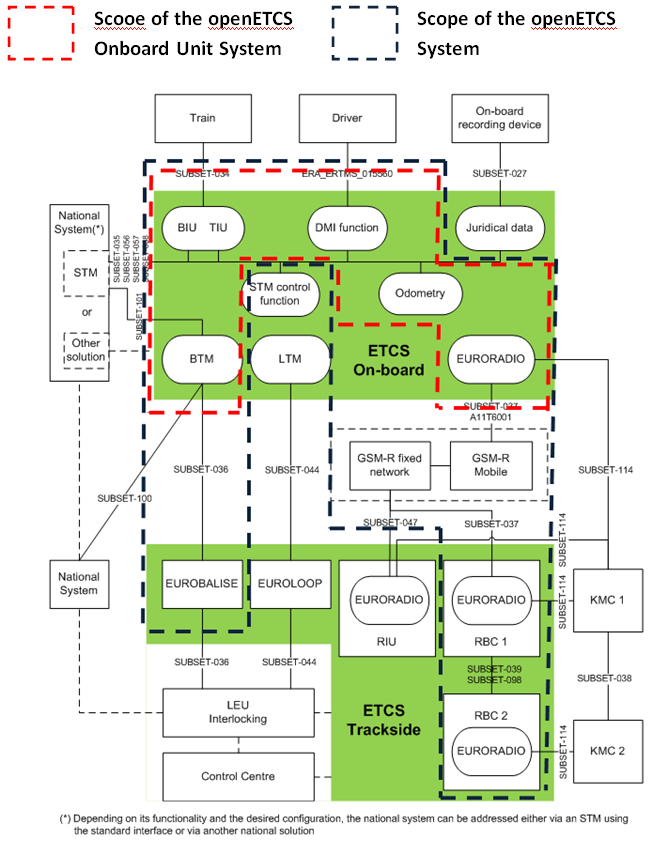
\includegraphics[scale=0.7]{images/ArchitectureSRS}
\caption{Scope of System according to ERA TSI Chapter 2}
\label{Scope of System according to ERA TSI Chapter 2}
\end{figure}

\section{System Architecture SysML View}
\textbf{The SysML System view of the architecture will reflect the scope accorgin to 4.1 and is a top down breakdown to the design layer. The functional breakdown has been done in Scade System and is part of the design model. Furthermore it will reflect all the external and internal interface that will will be described in 4.3. Another goal of the System Architecture SysML view is to explain and set the boundaries for the ETCS Kernel development "F2 Kernel" as the main design part of the openETCS@ITEA2 project.}

\subsection{1st level System Architecture view}
\textbf{All subystem of the ETCS/ERTMS Basic Sytem according in the scope of the openETCS@ITEA2 project will be reflected in this 1st level view. Furthermore the interlocking as part of a full Rail Signalling System, but not part of the openETCS scope, will be highlighted in this view.}

\textit{Interlocking =  interlocking is an arrangement of signal apparatus that prevents conflicting movements through an arrangement of tracks such as junctions or crossings. The signalling appliances and tracks are sometimes collectively referred to as an interlocking plant. An interlocking is designed so that it is impossible to display a signal to proceed unless the route to be used is proven safe.}


\begin{figure}[h]
\centering
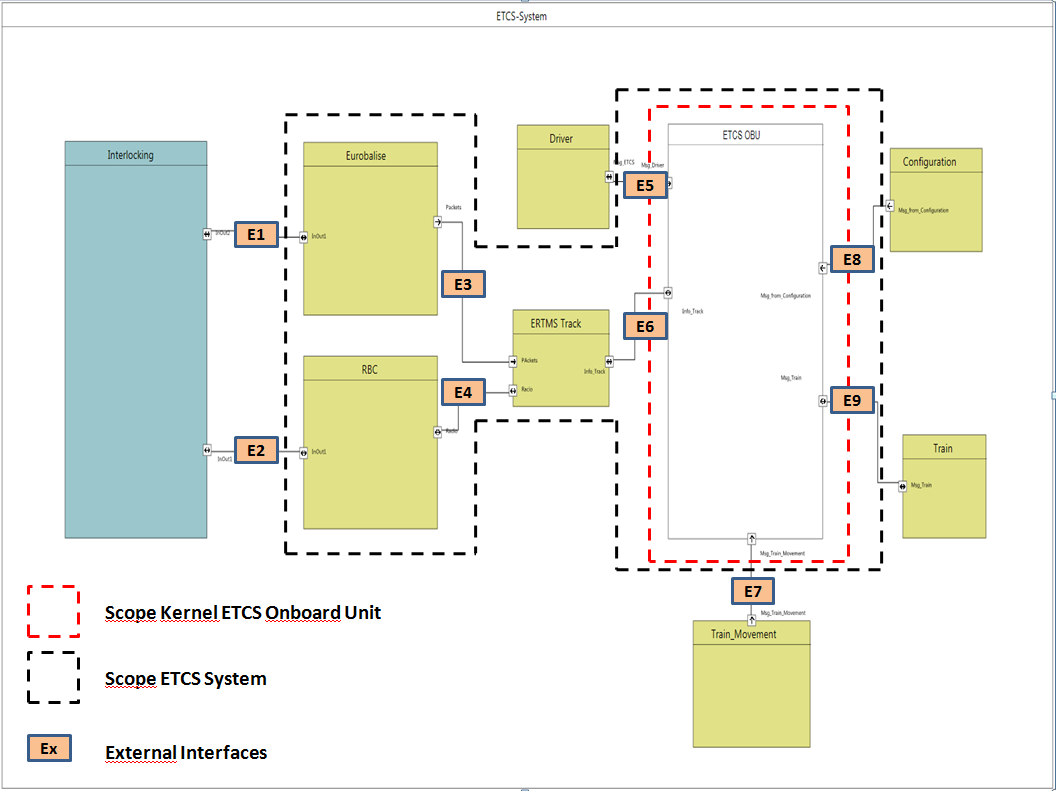
\includegraphics[scale=0.6]{images/1stlevelarchitecture}
\caption{1st level System Architecture view}
\label{1st level System Architecture view}
\end{figure}

\newpage
\subsection{2st level System Architecture view}
\textbf{The 2nd level system view will provide a decopmosition of the ETCS Onboard Unit systems and the Kernerl of the ETCS. The Kernel is the main part of the ETCS Onboard Unit system and reflects the functions specified in the ERA TSI Subset 26. Therefore the boundaries and interfaces to the other subasystems of the ETCS Onbard Unit needs to be fully desribed and formal. At least the formalisation kernel functions and boundaries should be realized in the openETCS project.}

\begin{figure}[h]
\centering
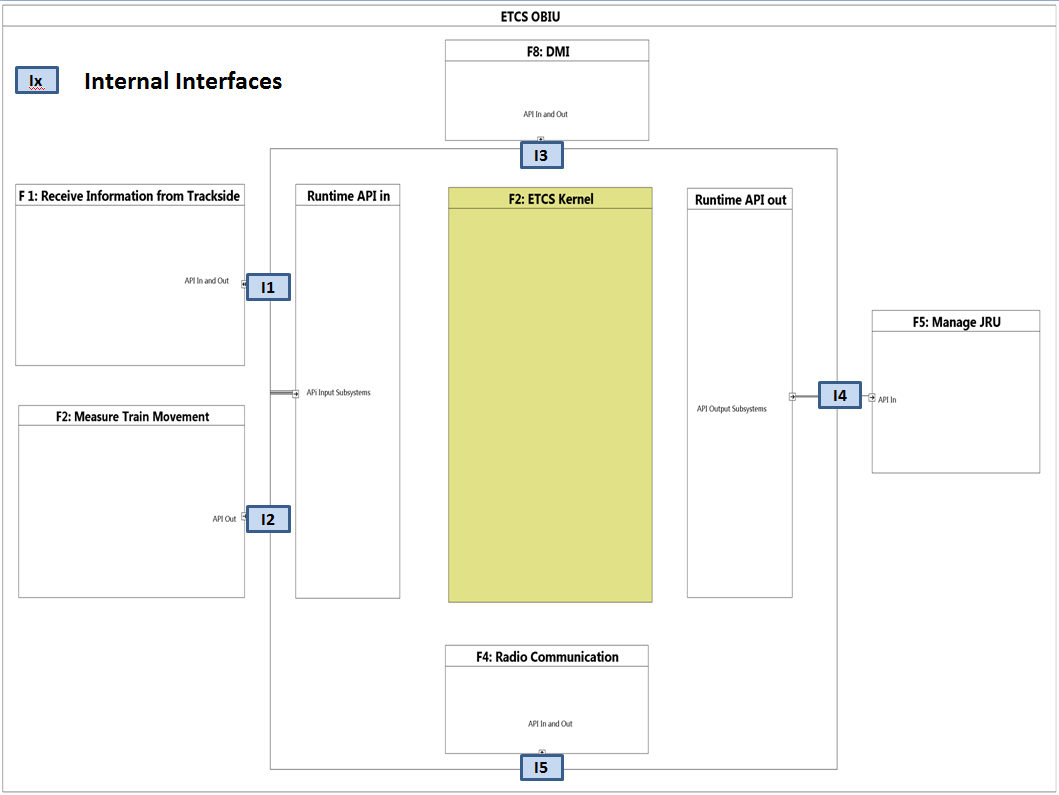
\includegraphics[scale=0.6]{images/2ndlevelarchitecture}
\caption{2nd level System Architecture view}
\label{2nd level System Architecture view}
\end{figure}

\subsection{3rd level System Architecture view}
\textbf{The 3rd level system view will provide a decopmosition of the ETCS Kernel of the ETCS Onboard Unit Systems. The decomposition and further design of the subfunctions of the kernel are part of the chapter 6 in this document. In chapter 6 we will consider the design description that will be completed by every designer itself. The designer can decided in this layer about the decomposition and boundaries of his subsystem, but need to describe the design choices.}

\newpage
\section{Interfaces}
\textbf{This section will consider the External and Internal interfaces as descibed in the system decomposition figures in 4.2.1 and 4.2.2}

\subsection{External Interfaces}
\textbf{External interfaces will describe the data flow between the Systems outside of the scope of the openETCS Project and the ETCS Onboard Unit System}

\paragraph*{E1:} In- and Out flow between the Interlocking an Eurobalise. There will be 2 kind of balises

\begin{itemize}
\item Fixed Balise: no interaction to the interlocking
\item Balise Controlled: interaction to the interlocking trough LEU
\end{itemize}

\begin{figure}[h]
\centering
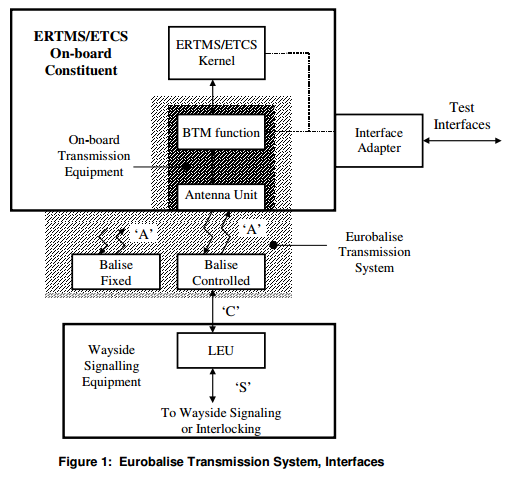
\includegraphics[scale=0.8]{images/Eurobalise}
\caption{Eurobalise}
\label{Eurobalise}
\end{figure}


\paragraph{E2:} In- and Out flow between the Interlocking and Radio Block Control.
This External interface will ensure the states or logics directly to the Radio Block Control and the other way back from the train to the interlocking.\\

\paragraph{E3:} Input flow from the Eurobalise to the Balise Transmission Module or Antenna Unit (BTM) into the ETCS Onboard Unit. As already described on the figure in E1.

\paragraph{E4:} In- and Out flow between the Radio Block Controll and the Euroradio Modul into the ETCS Onboard Unit. This interface is not in Level 0 or 1 active since there is no necessary for ETCS Radio interaction between track and train.

\paragraph{E5:} This interface will describe the interaction between the Human and Display (Human Machine Interface or Driver Machine Interface). 
See description on the figure below

\begin{figure}[h]
\centering
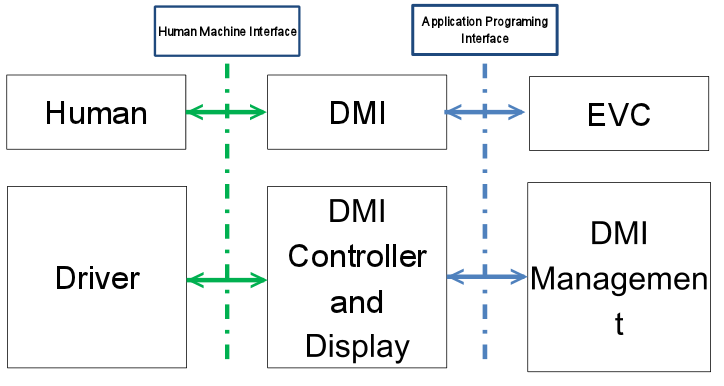
\includegraphics[scale=0.8]{images/DMIinterfaces}
\caption{DMI Interfaces}
\label{DMI Interfaces}
\end{figure}

\paragraph{E6:} This interface is composite the interfaces E3 and E4.

\paragraph{E7:} Input interface to the Odometrie Subsystem of the ETCS Onboard System. Will send information to train if there is any movemement outside the ETCS System is leading such as "cold movement".

\paragraph{E8:} Input interface to the ETCS Onboard Unit system to set configuration data such as fixed values, system values, national values and train configuration.

\paragraph{E9:} In- and Out flow between the ETCS Onboard Unit System and the Train. This interface will describe the itneraction between the Train and the ETCS Onboard Unit System such as brake controll, traction controll, door controll, ....

\subsection{Internal Interfaces}
\textbf{Internal interfaces will describe the data flow between the ETCS Onboard Unit Kernel and ETCS Onboard Unit Subsystems within the ETCS Onboard Unit System.}

\paragraph{I1:} In flow from the Balise Transmission Module (BTM or Antenna) to the "F2 ETCS Kernel" trough Runtime API in. Transmitted data are information from the Eurobalise.

\paragraph{I2:} In flow from the Odometrie (ODO) to the "F2 ETCS Kernel" trough Runtime API in. Transmitted data are information from the Movement of the train.

\paragraph{I3:} In- and Out flow between the DMI Controller and the "F2 ETCS Kernel" trough Runtime API in and out. Transmitted data are information of driver action and display. See description in figure of "External Interface E5".

\paragraph{I4:} Out flow from "F2 ETCS Kernel" to the JRU Manager trough Runtime API out. Transmitted data are all necessary information for a juridical recorder unit "black box".

\paragraph{I5:} In- and Out flow between the Euroradio and "F2 ETCS Kernel" trough Runtime API in and out. Transmitted data are radio track information (RBC) and information to the track (RBC). 

